\chapter{Two protocols based on Spekkens contextuality}

\section{Self-testing from approximately operationally equivalent preparations and bounded memory}
Let $n\geq 5$ be an odd integer. The protocol we consider is reminiscent of the ideal $n$-cycle reference experiment \ref{eqn:ncycleideal}. As such, we assume an experimenter to be able to freely choose between $n$ three-outcome measurements $\{M_i\}_{i=1}^n$ with outcomes $m_1$, $m_2$, $m_3$. We assume measurements to be chosen according to a uniform distribution and denote measurement events by $m_k\vert M_i,P_0 \equiv m_k\vert M_i$, or $m_k,m_l\vert M_i,M_j, P_0 \equiv m_k,m_l\vert M_i,M_j$ for two sequential measurements. As shown in Figure REF, for ideally operating devices, the measurement events $m_1 \vert M_i$ correspond to the rank-one projectors $\vert u_i^{(n)}\rangle\langle u_i^{(n)}\vert$. Further, in the ideal case, the measurement events $m_3\vert M_i\equiv m_1\vert M_{i\oplus 1}\equiv\vert u_{i\oplus 1}^{(n)}\rangle\langle u_{i\oplus 1}^{(n)}\vert$ and the events $m_2\vert M_i$ correspond to the projectors $\mathbb{1}-\vert u_i^{(n)}\rangle\langle u_i^{(n)}\vert-\vert u_{i\oplus 1}^{(n)}\rangle\langle u_{i\oplus 1}^{(n)}\vert$, projecting onto the pure qutrit state completing the orthogonal triad $\subset \mathbb{R}^3$. In Figure REF, the events $m_3 \vert M_i$ and $m_1\vert M_{i\oplus 1}$ are non-overlapping, despite corresponding to the same ideal projectors, to highlight we do not need to assume the operational equivalence of these.

\begin{figure}
	\begin{subfigure}[t]{0.55\textwidth}
    	\centering
    	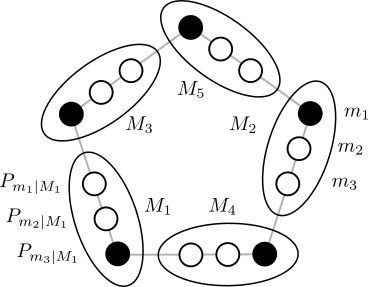
\includegraphics[width=\textwidth]{images/mntsandpreps.png}
        \caption{}
	\end{subfigure}
	\hfill
    \begin{subfigure}[t]{0.55\textwidth}
    	\centering 
        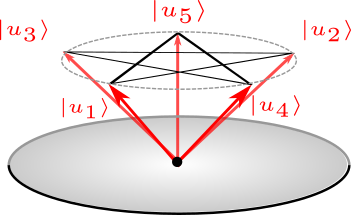
\includegraphics[width=0.8\textwidth]{images/kcbsrefstates.png}
        \caption{}
    \end{subfigure}
    \caption{}
\end{figure}

Like in Section REF, we assume i.i.d.\ rounds, i.e. the devices to operate in an identical manner for all rounds of the protocol, in particular independently of previous input-output cycles. This allows us to lift relative frequencies to probabilities. We will discuss all other assumptions in due time. The protocol consists of the following steps:
\begin{enumerate}
\item The experimenter prepares the system in a distinguished preparation $P_0$ by selecting the appropriate setting on the corresponding device.
\item The experimenter samples from a uniform distribution and selects two integers $(i,j)\in\{1,\dots,n\}^2$ at random.
\item The experimenter performs the measurements $M_i$, $M_j$ in sequence, first $M_i$, then $M_j$. He does so by selecting the correct settings on the corresponding devices and records the outcomes.
\item Steps 1-3 are repeated to obtain estimates for the probability distributions $p((m_k,m_l)\vert (M_i,M_j),P_0)$. 
\item Additionally, the experimenter performs single measurements on two auxilliary preparations $P_1$ and $P_2$ he can choose from and obtains estimates for the probability distributions $p(m_k\vert M,i, P_j)$, for $j\in{1,2}$.
\item Post-processing
	\begin{enumerate}
	\item Certify quantumness
	\item Bound compatible quantum models
	\end{enumerate}
\end{enumerate}

We write the free choice of measurements $(M_i,M_j)$ and subsequent outcomes $(m_k,m_l)$ as ordered lists to indicate that the distributions $p((m_k,m_l)\vert (M_i,M_j),P_0)$ are in general not independent of the order, since we do not assume any underlying compatibility relations, like we did in Section REF. In the ideal case, the distinguished preparation $P_0$ corresponds to the $\ket{0}$ qutrit state, which produces a maximal violation of the KCBS inequality. Additionally, we assume access to two additional auxilliary preparations, $P_1$ and $P_2$, which we require to establish approximate operational equivalences during post-processing. In the ideal case the preparations $P_1$ and $P_2$ correspond to the $\ket{1}$ and $\ket{2}$ qutrit states, forming an orthogonal triad with $P_0\equiv\ket{0}\bra{0}$. The convex combination $\frac{1}{3}\sum_{i=0}^2 P_i\equiv\frac{1}{3}\sum_{i=0}^2\ket{i}\bra{i}=\frac{\mathbb{1}}{3}$ corresponds to the fully mixed state $\frac{\mathbb{1}}{3}$, as does the convex combination with equal weights of the ideal projectors corresponding to the measurement events $\{m_k\vert M_i\}_{k=1}^3$ for all $i\in\{1,\dots,n\}$. Here, we implicitly defined the convex combination of two preparations to be the preparation that is implemented by generating a random number and performing the preparation procedure associated with that outcome. We note that Steps 1-4 of the protocol correspond almost one-to-one to the steps of the protocol in CITE, which was discussed in Section REF, the only difference being that the experimenter now freely chooses between $n^2$, as opposed to $n$ measurement settings.

We now elaborate on Step 6 of the protocol, detailing how an agent may post-process the acquired data, with the goal of self-testing the apparatus. The experimenter retrospectively defines $3n$ preparations, which we denote $\{P_{m_k\vert M_i}\}_{\substack{i\in\{1,\dots,n\} \\ k\in\{1,2,3\}}}$. As suggested by the notation, $P_{m_k\vert M_i}$ is prepared by performing the measurement $M_i$ on a system initially prepared like $P_0$, and conditioning on the outcome $m_k$. We refer to these preparations as retrospective, since they are not directly implemented by the experimenter. However, one can infer the relevant statistics $p(m_k\vert M_i, P_{m_l\vert M_j})$ for these preparations from the distributions $p((m_k,m_l)\vert (M_i,M_j))$:
\begin{equation}
p(m_k\vert M_i, P_{m_l\vert M_j})=\frac{p((m_k,m_l)\vert (M_i,M_j))}{\sum_{k'\in\{1,2,3\}} p((m_{k'},m_l)\vert (M_i,M_j))}.
\end{equation}
These retrospective preparations will be used in Section REF, where we propose a criterion to certify the quantumness of the apparatus.
\subsection{Step 6a: Certifying quantumness}
By coarse-graining, we obtain $3n$ binary measurements from the $n$ three-outcome measurements $M_i$. In total, we define $3n$ binary measurements and $3n$ preparations during post-processing. We denote the outcomes of the $3n$ binary measurements as $0$,$1$, where the outcome $0$ corresponds to the two coarse-grained measurement events. If we consider the ideal reference experiment REF and take the outcomes $0$, $1$ to be the eigenvalues of the binary projective measurements, one can think of these as rank-one projectors. There are $2n$ ideal binary measurements that probe the probability of finding the system in one of the $n$ one-dimensional subspaces spanned by the $n$ cycle states. The other $n$ ideal binary measurements correspond to rank-one projectors onto states in an orthogonal triad containing two cycle states. For the extent of this subsection we will for simplicity index the $3n$ binary measurements and preparations like $\{M_i\}_{i\in\{1,\dots,3n\}}$ and $\{P_i\}_{i\in\{1,\dots,3n\}}$, ordered such that the ideal measurement $M_i$